\clearpage

\section {Predictions of single $\mu$-like ring event reconstructed energy spectrum in SuperK}
\label{sec:spectrum_prediction}

\subsection {Methodology}

In this analysis, 
the oscillation parameters are determined 
by fitting the reconstructed energy ($E_{r}$) spectrum
of single $\mu$-like ring events observed at SuperK with the predicted spectrum.
The predicted number $N_{SK;r}$ 
of single $\mu$-like ring events in the $r^{th}$ reconstructed energy bin
is computed as follows:

\begin{equation}
\displaystyle
  N_{SK;r} = 
    \sum_{m} \sum_{t} \sum_{r\prime}
        P_{m;t} \cdot
        T_{r;r\prime;f_{E; r}^{SK}} \cdot
        S_{m;t;r\prime;\vec{f}} \cdot
        N_{SK;m;r\prime;t}^{MC} \cdot
\label{eq:far_prediction}
\end{equation}

In Eq.~\ref{eq:far_prediction}, $N_{SK;m;r\prime;t}^{MC}$ is the input SuperK Monte Carlo (MC) template 
containing the number of events in the single $\mu$-like ring MC sample with true reaction mode $m$ in the 
true energy bin t and the reconstructed energy bin $r\prime$.
The construction of the nominal MC templates is discussed in Sec.~\ref{sec:mc_templates}.
Both flux-tuning weights based on NA61 hadron-production data (see Sec.~\ref{sec:na61_weights})
and flux and cross-section tuning weights based on ND280 data (see Sec.~\ref{sec:banff_weights})
are applied to the nominal MC templates.
$S_{m;t;r\prime;\vec{f}}$ is an overall, multiplicative, systematic error factor 
depending on the reaction mode $m$, the true energy bin $t$, the reconstructed energy bin $r\prime$ 
and a vector of nuisance (systematic) parameters $\vec{f}$. 
A complete description of the nuisance parameters considered in this analysis is given in Sec.~\ref{sec:systematics}.
$T_{r;r\prime;f_{E; r}^{SK}}$ is a transfer function describing the migration of events
between the reconstructed energy bins $r$ and $r\prime$ due to uncertainty in the SuperK reconstructed energy
scale, expressed here in terms of the nuisance parameter $f_{E; r}^{SK}$.
Finally, $P_{m;t}$ is the 3-flavour oscillation probability applied to the true energy
bin t of the SuperK MC template which corresponds to mode $m$;
application of the term $P_{m;t}$ is discussed in Sec.~\ref{sec:applying_oscillations}.

%....................................................................................................................
%....................................................................................................................

\subsection {Construction of nominal SuperK Monte Carlo templates}
\label{sec:mc_templates}

The nominal SuperK single $\mu$-like ring MC templates $N_{SK;m;r;t}^{MC}$
are constructed by applying the single $\mu$-like ring selection cuts to the official SuperK MC samples.
Details of the MC samples are given in Sec.~\ref{sec:mc_templates:input_mc}.
The calculation of the normalisation of each MC sample is described in Sec.~\ref{sec:mc_templates:normalization}.
The official single $\mu$-like ring selection cuts are listed in Sec.~\ref{sec:mc_templates:1Rmu_cuts}.
The list of MC templates used in this analysis is shown in Sec.~\ref{sec:mc_templates:template_list},
while the true and reconstructed energy binning of the templates is discussed 
in Sec.~\ref{sec:mc_templates:template_binning}.

%....................................................................................................................
\subsubsection {Input Monte Carlo samples}
\label{sec:mc_templates:input_mc}


This analysis uses the official 14a SuperK MC samples. These were generated using the 13a JNUBEAM flux, NEUT 5.3.2, 
SKDETSIM v13p90 and the 14b SuperK software \cite{SuperkMC14a}. Six MC samples were generated for antineutrino beam 
mode running (horn current -250kA). Four of the samples ($\bar{\nu}_{\mu}$, $\nu_{\mu}$, $\bar{\nu}_{e}$ and $\nu_{e}$) 
were generated using the nominal JNUBEAM flux without oscillations.
The fifth sample is $\bar{\nu}_{e}$ interactions generated with the $\bar{\nu}_{\mu}$ flux, and will be denoted the 
``oscillated $\bar{\nu}_{e}$'' sample (it corresponds to the ``signal-$\bar{\nu}_{e}$'' sample in the 
$\bar{\nu}_{e}$-appearance analysis). The sixth sample is $\nu_{e}$ interactions generated with the $\nu_{\mu}$ flux, 
and will be denoted the ``oscillated $\nu_{e}$'' sample.

%....................................................................................................................
\subsubsection {Normalisation of Monte Carlo samples}
\label{sec:mc_templates:normalization}


The normalisation (integrated exposure in terms of POT) of each event sample is calculated from
the number of events with a MC truth interaction vertex within the 22.5 kt fiducial volume.

\begin{equation}
\displaystyle
  N = \int  dS dI dE \cdot
            \frac{d^{3}\Phi_{SK}}{dS dI dE_{\nu}} \cdot
            \sigma_{H_{2}O} \cdot
            \frac{N_{A}}{A} \cdot \rho \cdot L 
\end{equation}
where 
$d^{3}\Phi_{SK}$/$dS dI dE$ is the number of flux particles for the given neutrino species 
per neutrino energy bin $dE_{\nu}$, per unit area $dS$ and per POT,
$\sigma_{H_{2}O}$ is the total interaction cross section in water
for the given neutrino species,
I is the beam intensity in terms of POT,
$N_{A}$ is  Avogadro's number,
$A$ is the mass number for water,
$\rho$ is the water density
and L is the neutrino path length in the water volume.

The SuperK MC samples are normalised to the Run 5+6 POT (\TotalPot) using the numbers in Tab.~\ref{tab:SKMCNormalisation}. 
Assuming that all the MC files are used, each sample is first normalised to 10$^{21}$ POT by weighting it 
with the ratio of the number of events per 22.5 kt per $10^{21}$ POT (second column) to the number of generated 
events in the true fiducial volume in all the available MC (third column). Then each sample is 
normalised to \TotalPot{} POT by weighting the result by \TotalPotPerTwentyOne (the Run 5+6 POT in units of $10^{21}$ POT). 
\begin{table}
\centering
\begin{tabular}{| c | c | c |}
\hline
Sample                        &  Number of events     & Number of generated events \\
                              & per 22.5 kt fiducial  & in true fiducial volume    \\
                              & per $10^{21}$ POT     & in all available MC        \\  
\hline             
$\bar{\nu}_{\mu}$             &     353.789           &       633988               \\
$\nu_{\mu}$                   &     208.369           &       634659               \\
$\bar{\nu}_{e}$               &      6.811            &       127013               \\
$\nu_{e}$                     &      8.941            &       127262               \\
Oscillated $\bar{\nu}_{e}$    &     376.420           &       126812               \\
Oscillated $\nu_{e}$          &     215.099           &       127278               \\
\hline
\end{tabular}
\caption{
  Normalisation of input SuperK MC samples \cite{SuperkMC14a}
}
\label{tab:SKMCNormalisation}
\end{table}

%....................................................................................................................
\subsubsection {Single $\mu$-like ring event selection cuts}
\label{sec:mc_templates:1Rmu_cuts}

The SuperK MC templates contain events from the 
$\nu_{\mu}$, $\bar{\nu}_{\mu}$, $\nu_{e}$, $\bar{\nu}_{e}$, oscillated $\nu_{e}$ and oscillated $\bar{\nu}_{e}$ 
 samples passing the standard SuperK selection cuts for single $\mu$-like ring events.
These cuts are:

\begin{itemize}
\item
the number of PMT hits in the highest-charge OD cluster is less than or
equal to 15, and the event passes the flasher rejection cuts
({\tt evclass == 1}),
\item
the reconstructed vertex is at least 2 metres away from the ID wall 
({\tt wall $>$ 200}),
\item
the visible energy in the event is above 30 MeV 
({\tt evis  $>$ 30}),
\item
there is exactly 1 reconstructed ring in the event 
({\tt nring == 1}),
\item
the reconstructed ring is $\mu$-like 
({\tt ip[0] = 3}),
\item
the reconstructed muon momentum is above 200 MeV 
({\tt amomm[0] $>$ 200}), and
\item
there is at most 1 decay e$^{-}$ in the event 
({\tt nmue $<$= 1}).
\end{itemize}

%....................................................................................................................
\subsubsection {List of Monte Carlo templates}
\label{sec:mc_templates:template_list}

For each SuperK MC sample, a number of different MC templates is constructed 
corresponding to different true reaction modes.
The template granularity depends on the type of oscillation analysis and the specific 
systematic parameters considered in the analysis.
12 MC templates were used for our 2010 Run 1+2 2-flavour disappearance analysis \cite{OurRun12DisappAnalysis}, while
15 MC templates were used for our 2010 Run 1+2 3-flavour disappearance analysis \cite{OurRun12DisappAnalysis3Flavour},
28 MC templates were used for our 2012 Run 1+2+3 3-flavour disappearance analysis \cite{OurRun123DisappAnalysis3Flavour} and
32 MC templates were used for our 2014 Run 1+2+3+4 3-flavour disappearance analysis \cite{OurRun1234DisappAnalysis3Flavour}.

In our previous $\nu_{\mu}$-disappearance analyses, NC events were divided into NC1$\pi^{\pm}$ and NC other. For this 
$\bar{\nu}_{\mu}$-disappearance analysis, the NC interaction modes have been further subdivided into NC1$\pi^{\pm}$, 
NC1$\pi^{0}$, NC coherent and NC other. We have also added 5 CC MEC templates for $\bar{\nu}_{\mu}$, $\nu_{\mu}$, $\bar{\nu}_{e}$, 
$\nu_{e}$ and oscillated $\nu_{e}$ and 5 templates for the oscillated $\bar{\nu}_{e}$ MC sample. This gives a 
total of \NMCTemplate{} templates: 
\begin{itemize}
\item  $\bar{\nu}_{\mu}$ CCQE,
\item  $\bar{\nu}_{\mu}$ CC MEC,
\item  $\bar{\nu}_{\mu}$ CC1$\pi$,
\item  $\bar{\nu}_{\mu}$ CC coherent,
\item  $\bar{\nu}_{\mu}$ CC other,
\item  $\bar{\nu}_{\mu}$(and $\rightarrow$ $\bar{\nu}_{e}$, $\bar{\nu}_{\tau}$) NC1$\pi^{\pm}$,
\item  $\bar{\nu}_{\mu}$(and $\rightarrow$ $\bar{\nu}_{e}$, $\bar{\nu}_{\tau}$) NC1$\pi^{0}$,
\item  $\bar{\nu}_{\mu}$(and $\rightarrow$ $\bar{\nu}_{e}$, $\bar{\nu}_{\tau}$) NC coherent,
\item  $\bar{\nu}_{\mu}$(and $\rightarrow$ $\bar{\nu}_{e}$, $\bar{\nu}_{\tau}$) NC other,
\item  $\nu_{\mu}$ CCQE,
\item  $\nu_{\mu}$ CC MEC,
\item  $\nu_{\mu}$ CC1$\pi$, 
\item  $\nu_{\mu}$ CC coherent, 
\item  $\nu_{\mu}$ CC other, 
\item  $\nu_{\mu}$ (and $\rightarrow$ $\nu_{e}$, $\nu_{\tau}$) NC1$\pi^{\pm}$, 
\item  $\nu_{\mu}$ (and $\rightarrow$ $\nu_{e}$, $\nu_{\tau}$) NC1$\pi^{0}$,
\item  $\nu_{\mu}$ (and $\rightarrow$ $\nu_{e}$, $\nu_{\tau}$) NC coherent,
\item  $\nu_{\mu}$ (and $\rightarrow$ $\nu_{e}$, $\nu_{\tau}$) NC other, 
\item  $\bar{\nu}_{e}$ CCQE,
\item  $\bar{\nu}_{e}$ CC MEC,
\item  $\bar{\nu}_{e}$ CC1$\pi$,
\item  $\bar{\nu}_{e}$ CC coherent,
\item  $\bar{\nu}_{e}$ CC other,
\item  $\bar{\nu}_{e}$ (and $\rightarrow$ $\bar{\nu}_{\mu}$, $\bar{\nu}_{\tau}$) NC1$\pi^{\pm}$,
\item  $\bar{\nu}_{e}$ (and $\rightarrow$ $\bar{\nu}_{\mu}$, $\bar{\nu}_{\tau}$) NC1$\pi^{0}$,
\item  $\bar{\nu}_{e}$ (and $\rightarrow$ $\bar{\nu}_{\mu}$, $\bar{\nu}_{\tau}$) NC coherent,
\item  $\bar{\nu}_{e}$ (and $\rightarrow$ $\bar{\nu}_{\mu}$, $\bar{\nu}_{\tau}$) NC other,
\item  $\nu_{e}$ CCQE, 
\item  $\nu_{e}$ CC MEC,
\item  $\nu_{e}$ CC1$\pi$,
\item  $\nu_{e}$ CC coherent,
\item  $\nu_{e}$ CC other,
\item  $\nu_{e}$ (and $\rightarrow$ $\nu_{\mu}$, $\nu_{\tau}$) NC1$\pi^{\pm}$,
\item  $\nu_{e}$ (and $\rightarrow$ $\nu_{\mu}$, $\nu_{\tau}$) NC1$\pi^{0}$,
\item  $\nu_{e}$ (and $\rightarrow$ $\nu_{\mu}$, $\nu_{\tau}$) NC coherent,
\item  $\nu_{e}$ (and $\rightarrow$ $\nu_{\mu}$, $\nu_{\tau}$) NC other,
\item  oscillated $\nu_{\mu} \rightarrow \nu_{e}$ CCQE,
\item  oscillated $\nu_{\mu} \rightarrow \nu_{e}$ CC MEC,
\item  oscillated $\nu_{\mu} \rightarrow \nu_{e}$ CC1$\pi$,
\item  oscillated $\nu_{\mu} \rightarrow \nu_{e}$ CC coherent,
\item  oscillated $\nu_{\mu} \rightarrow \nu_{e}$ CC other,
\item  oscillated $\bar{\nu}_{\mu} \rightarrow \bar{\nu}_{e}$ CCQE,
\item  oscillated $\bar{\nu}_{\mu} \rightarrow \bar{\nu}_{e}$ CC MEC,
\item  oscillated $\bar{\nu}_{\mu} \rightarrow \bar{\nu}_{e}$ CC1$\pi$,
\item  oscillated $\bar{\nu}_{\mu} \rightarrow \bar{\nu}_{e}$ CC coherent,
\item  oscillated $\bar{\nu}_{\mu} \rightarrow \bar{\nu}_{e}$ CC other.
%\item  oscillated $\bar{\nu}_{e} \rightarrow \bar{\nu}_{\mu}$ CCQE,
%\item  oscillated $\bar{\nu}_{e} \rightarrow \bar{\nu}_{\mu}$ CC MEC
%\item  oscillated $\bar{\nu}_{e} \rightarrow \bar{\nu}_{\mu}$ CC1$\pi$,
%\item  oscillated $\bar{\nu}_{e} \rightarrow \bar{\nu}_{\mu}$ CC coherent, and
%\item  oscillated $\bar{\nu}_{e} \rightarrow \bar{\nu}_{\mu}$ CC other.
%\item  oscillated $\nu_{e} \rightarrow \nu_{\mu}$ CCQE,
%\item  oscillated $\nu_{e} \rightarrow \nu_{\mu}$ CC MEC,
%\item  oscillated $\nu_{e} \rightarrow \nu_{\mu}$ CC1$\pi$,
%\item  oscillated $\nu_{e} \rightarrow \nu_{\mu}$ CC coherent, and
%\item  oscillated $\nu_{e} \rightarrow \nu_{\mu}$ CC other.
\end{itemize}

\begin{table}
\begin{tabular} { | c ||c | c | c | c |  | }
\hline
                                                  & Nominal MC          & Flux-tuned MC       & BANFF prefit MC     & BANFF postfit MC     \\
                                                  &                     &                     & (flux + NIWG tune)  &                      \\ \hline  
Total                                             & 96.434              & 100.439             & 87.615              & 103.604              \\ \hline 
\hline 
$\nu_\mu$ CCQE                                    & 14.186              & 14.493              & 14.250              & 15.405               \\ \hline 
$\nu_\mu$ CC 1$\pi$                               & 4.792               & 5.019               & 5.019               & 3.666                \\ \hline 
$\nu_\mu$ CC coherent                             & 0.201               & 0.212               & 0.212               & 0.244                \\ \hline 
$\nu_\mu$ CC MEC                                  & 2.630               & 2.707               & 0.731               & 3.022                \\ \hline 
$\nu_\mu$ CC other                                & 1.198               & 1.307               & 1.307               & 1.393                \\ \hline 
$\nu_\mu$/$\nu_\tau$ NC 1$\pi^{+/-}$              & 0.495               & 0.523               & 0.523               & 0.340                \\ \hline 
$\nu_\mu$/$\nu_\tau$ NC 1$\pi^0$                  & 0.081               & 0.086               & 0.086               & 0.051                \\ \hline 
$\nu_\mu$/$\nu_\tau$ NC coherent                  & 0.001               & 0.001               & 0.001               & 0.001                \\ \hline 
$\nu_\mu$/$\nu_\tau$ NC other                     & 0.434               & 0.470               & 0.470               & 0.705                \\ \hline 
$\bar{\nu}_\mu$ CCQE                              & 53.188              & 55.834              & 50.852              & 57.962               \\ \hline 
$\bar{\nu}_\mu$ CC 1$\pi$                         & 7.506               & 7.658               & 7.658               & 6.746                \\ \hline 
$\bar{\nu}_\mu$ CC coherent                       & 2.409               & 2.515               & 2.515               & 3.082                \\ \hline 
$\bar{\nu}_\mu$ CC MEC                            & 7.382               & 7.699               & 2.079               & 9.037                \\ \hline 
$\bar{\nu}_\mu$ CC other                          & 0.914               & 0.891               & 0.891               & 1.005                \\ \hline 
$\bar{\nu}_\mu$/$\bar{\nu}_\tau$ NC 1$\pi^{+/-}$  & 0.571               & 0.581               & 0.581               & 0.381                \\ \hline 
$\bar{\nu}_\mu$/$\bar{\nu}_\tau$ NC 1$\pi^0$      & 0.081               & 0.082               & 0.082               & 0.048                \\ \hline 
$\bar{\nu}_\mu$/$\bar{\nu}_\tau$ NC coherent      & 0.006               & 0.006               & 0.006               & 0.007                \\ \hline 
$\bar{\nu}_\mu$/$\bar{\nu}_\tau$ NC other         & 0.265               & 0.260               & 0.260               & 0.410                \\ \hline 
$\nu_e$ CCQE                                      & 0.003               & 0.004               & 0.003               & 0.004                \\ \hline 
$\nu_e$ CC 1$\pi$                                 & 0.003               & 0.003               & 0.003               & 0.003                \\ \hline 
$\nu_e$ CC coherent                               & 0.000               & 0.000               & 0.000               & 0.000                \\ \hline 
$\nu_e$ CC MEC                                    & 0.001               & 0.001               & 0.000               & 0.001                \\ \hline 
$\nu_e$ CC other                                  & 0.001               & 0.001               & 0.001               & 0.001                \\ \hline 
$\nu_e$ NC 1$\pi^{+/-}$                           & 0.021               & 0.021               & 0.021               & 0.014                \\ \hline 
$\nu_e$ NC 1$\pi^0$                               & 0.003               & 0.004               & 0.004               & 0.002                \\ \hline 
$\nu_e$ NC coherent                               & 0.000               & 0.000               & 0.000               & 0.000                \\ \hline 
$\nu_e$ NC other                                  & 0.022               & 0.022               & 0.022               & 0.035                \\ \hline 
Osc. $\nu_e$ CCQE                                 & 0.000               & 0.000               & 0.000               & 0.000                \\ \hline 
Osc. $\nu_e$ CC 1$\pi$                            & 0.000               & 0.000               & 0.000               & 0.000                \\ \hline 
Osc. $\nu_e$ CC coherent                          & 0.000               & 0.000               & 0.000               & 0.000                \\ \hline 
Osc. $\nu_e$ CC MEC                               & 0.000               & 0.000               & 0.000               & 0.000                \\ \hline 
Osc. $\nu_e$ CC other                             & 0.000               & 0.000               & 0.000               & 0.000                \\ \hline 
$\bar{\nu}_e$ CCQE                                & 0.005               & 0.005               & 0.004               & 0.005                \\ \hline 
$\bar{\nu}_e$ CC 1$\pi$                           & 0.002               & 0.002               & 0.002               & 0.002                \\ \hline 
$\bar{\nu}_e$ CC coherent                         & 0.000               & 0.000               & 0.000               & 0.001                \\ \hline 
$\bar{\nu}_e$ CC MEC                              & 0.001               & 0.001               & 0.000               & 0.001                \\ \hline 
$\bar{\nu}_e$ CC other                            & 0.000               & 0.000               & 0.000               & 0.000                \\ \hline 
$\bar{\nu}_e$ NC 1$\pi^{+/-}$                     & 0.016               & 0.016               & 0.016               & 0.010                \\ \hline 
$\bar{\nu}_e$ NC 1$\pi^0$                         & 0.002               & 0.002               & 0.002               & 0.001                \\ \hline 
$\bar{\nu}_e$ NC coherent                         & 0.000               & 0.000               & 0.000               & 0.000                \\ \hline 
$\bar{\nu}_e$ NC other                            & 0.011               & 0.011               & 0.011               & 0.017                \\ \hline 
Osc. $\bar{\nu}_e$ CCQE                           & 0.000               & 0.000               & 0.000               & 0.000                \\ \hline 
Osc. $\bar{\nu}_e$ CC 1$\pi$                      & 0.000               & 0.000               & 0.000               & 0.000                \\ \hline 
Osc. $\bar{\nu}_e$ CC coherent                    & 0.000               & 0.000               & 0.000               & 0.000                \\ \hline 
Osc. $\bar{\nu}_e$ CC MEC                         & 0.000               & 0.000               & 0.000               & 0.000                \\ \hline 
Osc. $\bar{\nu}_e$ CC other                       & 0.000               & 0.000               & 0.000               & 0.000                \\ \hline 

\end{tabular}
\caption{
  Calculated predicted numbers of 1-ring $\mu$-like events without oscillations using the nominal MC templates, the
  NA61-tuned MC templates, the NIWG-tuned MC templates and the BANFF-tuned MC templates.
  The BANFF prefit column is the NA61 tuned data, with the CCQE samples reweighted according to the NIWG's external data fits~\cite{NIWGCCQE}.
  The total numbers of events and the numbers of events from each mode considered in this analysis are shown.
  These numbers were calculated for an exposure of \TotalPot POT.
}
\label{tab:nsk_nominal_no_osc}
\end{table}

%________________________________________________________________________________________________________________________________________________________________________________
\begin{table}
\begin{tabular} { | c ||c | c | c | c |  | }
\hline
                                                  & $N_{SK}$            & $N_{SK}$            & $N_{SK}$            & $N_{SK}$             \\ 
                                                  & Nominal MC          & Flux-tuned MC       & BANFF prefit MC     & BANFF postfit MC     \\
                                                  &                     &                     & (flux + NIWG tune)  &                      \\ \hline 
Total                                             & 33.161              & 34.240              & 30.715              & 34.584               \\ \hline  
\hline 
$\nu_\mu$ CCQE                                    & 6.269               & 6.525               & 6.447               & 6.871                \\ \hline 
$\nu_\mu$ CC 1$\pi$                               & 3.155               & 3.349               & 3.349               & 2.415                \\ \hline 
$\nu_\mu$ CC coherent                             & 0.136               & 0.146               & 0.146               & 0.167                \\ \hline 
$\nu_\mu$ CC MEC                                  & 1.365               & 1.428               & 0.386               & 1.578                \\ \hline 
$\nu_\mu$ CC other                                & 1.049               & 1.150               & 1.150               & 1.223                \\ \hline 
$\nu_\mu$/$\nu_\tau$ NC 1$\pi^{+/-}$              & 0.495               & 0.523               & 0.523               & 0.340                \\ \hline 
$\nu_\mu$/$\nu_\tau$ NC 1$\pi^0$                  & 0.081               & 0.086               & 0.086               & 0.051                \\ \hline 
$\nu_\mu$/$\nu_\tau$ NC coherent                  & 0.001               & 0.001               & 0.001               & 0.001                \\ \hline 
$\nu_\mu$/$\nu_\tau$ NC other                     & 0.434               & 0.470               & 0.470               & 0.705                \\ \hline 
$\bar{\nu}_\mu$ CCQE                              & 12.222              & 12.584              & 11.656              & 13.278               \\ \hline 
$\bar{\nu}_\mu$ CC 1$\pi$                         & 3.556               & 3.552               & 3.552               & 3.048                \\ \hline 
$\bar{\nu}_\mu$ CC coherent                       & 0.565               & 0.574               & 0.574               & 0.697                \\ \hline 
$\bar{\nu}_\mu$ CC MEC                            & 1.978               & 2.015               & 0.544               & 2.350                \\ \hline 
$\bar{\nu}_\mu$ CC other                          & 0.805               & 0.782               & 0.782               & 0.881                \\ \hline 
$\bar{\nu}_\mu$/$\bar{\nu}_\tau$ NC 1$\pi^{+/-}$  & 0.571               & 0.581               & 0.581               & 0.381                \\ \hline 
$\bar{\nu}_\mu$/$\bar{\nu}_\tau$ NC 1$\pi^0$      & 0.081               & 0.082               & 0.082               & 0.048                \\ \hline 
$\bar{\nu}_\mu$/$\bar{\nu}_\tau$ NC coherent      & 0.006               & 0.006               & 0.006               & 0.007                \\ \hline 
$\bar{\nu}_\mu$/$\bar{\nu}_\tau$ NC other         & 0.265               & 0.260               & 0.260               & 0.410                \\ \hline 
$\nu_e$ CCQE                                      & 0.003               & 0.003               & 0.003               & 0.004                \\ \hline 
$\nu_e$ CC 1$\pi$                                 & 0.003               & 0.003               & 0.003               & 0.003                \\ \hline 
$\nu_e$ CC coherent                               & 0.000               & 0.000               & 0.000               & 0.000                \\ \hline 
$\nu_e$ CC MEC                                    & 0.001               & 0.001               & 0.000               & 0.001                \\ \hline 
$\nu_e$ CC other                                  & 0.001               & 0.001               & 0.001               & 0.001                \\ \hline 
$\nu_e$ NC 1$\pi^{+/-}$                           & 0.021               & 0.021               & 0.021               & 0.014                \\ \hline 
$\nu_e$ NC 1$\pi^0$                               & 0.003               & 0.004               & 0.004               & 0.002                \\ \hline 
$\nu_e$ NC coherent                               & 0.000               & 0.000               & 0.000               & 0.000                \\ \hline 
$\nu_e$ NC other                                  & 0.022               & 0.022               & 0.022               & 0.035                \\ \hline 
Osc. $\nu_e$ CCQE                                 & 0.007               & 0.007               & 0.006               & 0.007                \\ \hline 
Osc. $\nu_e$ CC 1$\pi$                            & 0.003               & 0.003               & 0.003               & 0.003                \\ \hline 
Osc. $\nu_e$ CC coherent                          & 0.000               & 0.000               & 0.000               & 0.000                \\ \hline 
Osc. $\nu_e$ CC MEC                               & 0.001               & 0.001               & 0.000               & 0.001                \\ \hline 
Osc. $\nu_e$ CC other                             & 0.000               & 0.000               & 0.000               & 0.000                \\ \hline 
$\bar{\nu}_e$ CCQE                                & 0.005               & 0.005               & 0.004               & 0.005                \\ \hline 
$\bar{\nu}_e$ CC 1$\pi$                           & 0.002               & 0.002               & 0.002               & 0.002                \\ \hline 
$\bar{\nu}_e$ CC coherent                         & 0.000               & 0.000               & 0.000               & 0.000                \\ \hline 
$\bar{\nu}_e$ CC MEC                              & 0.001               & 0.001               & 0.000               & 0.001                \\ \hline 
$\bar{\nu}_e$ CC other                            & 0.000               & 0.000               & 0.000               & 0.000                \\ \hline 
$\bar{\nu}_e$ NC 1$\pi^{+/-}$                     & 0.016               & 0.016               & 0.016               & 0.010                \\ \hline 
$\bar{\nu}_e$ NC 1$\pi^0$                         & 0.002               & 0.002               & 0.002               & 0.001                \\ \hline 
$\bar{\nu}_e$ NC coherent                         & 0.000               & 0.000               & 0.000               & 0.000                \\ \hline 
$\bar{\nu}_e$ NC other                            & 0.011               & 0.011               & 0.011               & 0.017                \\ \hline 
Osc. $\bar{\nu}_e$ CCQE                           & 0.015               & 0.016               & 0.015               & 0.017                \\ \hline 
Osc. $\bar{\nu}_e$ CC 1$\pi$                      & 0.003               & 0.004               & 0.004               & 0.003                \\ \hline 
Osc. $\bar{\nu}_e$ CC coherent                    & 0.001               & 0.001               & 0.001               & 0.002                \\ \hline 
Osc. $\bar{\nu}_e$ CC MEC                         & 0.002               & 0.002               & 0.001               & 0.003                \\ \hline 
Osc. $\bar{\nu}_e$ CC other                       & 0.000               & 0.000               & 0.000               & 0.000                \\ \hline 

\end{tabular}
\caption{
  Calculated predicted numbers of 1-ring $\mu$-like events with oscillations using the nominal MC templates, the
  NA61-tuned MC templates, the NIWG-tuned MC templates and the BANFF-tuned MC templates.
  The BANFF prefit column is the NA61 tuned data, with the CCQE samples reweighted according to the NIWG's external data fits~\cite{NIWGCCQE}.
  The total numbers of events and the numbers of events from each mode considered in this analysis are shown.
  The normal hierarchy was assumed, with oscillation parameters give the values listed in table~\ref{tab:osc_params_fixed_values_reactor}.
  These numbers were calculated for an exposure of \TotalPot POT.
}
\label{tab:nsk_nominal_osc}
\end{table}


%....................................................................................................................
\subsubsection {Binning of Monte Carlo templates}
\label{sec:mc_templates:template_binning}

Each of the \NMCTemplate{}  MC templates has 6132 2-dimensional bins (= 84 true energy bins $\times$ 73 reconstructed energy bins).
The 84 true energy bins are arranged as follows:
\begin{itemize}
 \item   6 50-MeV bins from 0-0.3 GeV, 
 \item   28 25-MeV bins from 0.3-1 GeV, 
 \item   40 50-MeV bins from 1-3 GeV, 
 \item   5 100-MeV bin from 3-3.5 GeV, 
 \item   1 bin from 3.5-4 GeV, 
 \item   1 bin from 4-5 GeV, 
 \item   1 bin from 5-7 GeV, 
 \item   1 bin from 7-10 GeV and
 \item   1 bin from 10-30 GeV.
\end{itemize}

The 73 reconstructed energy bins are the following:
\begin{itemize}
 \item   60 50-MeV bins from 0-3 GeV, 
 \item   4 250-MeV bins from 3-4 GeV, 
 \item   4 500-MeV bins from 4-6 GeV, 
 \item   4 1000-MeV bins from 6-10 GeV and
 \item   1 bin from 10-30 GeV.
\end{itemize}
The same reconstructed neutrino energy binning is used for the fit of the single $\mu$-like ring reconstructed energy spectrum.

A study was performed to decide the optimum binning scheme balancing the needs for accuracy and speed.
Details are given in Appendix I of Ref.\ \cite{OurRun123DisappAnalysis3Flavour}.

The binning described here is unchanged with respect to the Run 1+2+3+4 $\nu_{\mu}$-disappearance analysis,


%....................................................................................................................
%....................................................................................................................
\subsection {Applying flux tuning based on NA61 data}
\label{sec:na61_weights}

In this analysis, the nominal MC templates, which were constructed using a MC event sample generated with the 13a flux,
are reweighted to the 13av1.1 flux (Run 5c-6e, June release) which was tuned on NA61 hadron production measurements \cite{FluxTuning13a}\cite{NA61T2K2014}.
The reweighted MC templates are denoted the {\em NA61-tuned} MC templates in this document.
The applied weights were obtained from \cite{FluxTuning13a} and are shown as a function of the true neutrino energy 
in Figs.~\ref{fig:na61_weights:numu}-\ref{fig:na61_weights:nuebar}.
The effect of this flux tune on the predicted reconstructed energy spectrum of 
single $\mu$-like ring events is discussed in Sec.~\ref{sec:nominal_and_tuned_predictions} 
(see Figs.~\ref{fig:na61_weights:numu}).
% and Tabs.\ {\color{red}???}). 

\begin{figure*}[htb]
\begin{minipage}[t]{0.48\linewidth}
\center
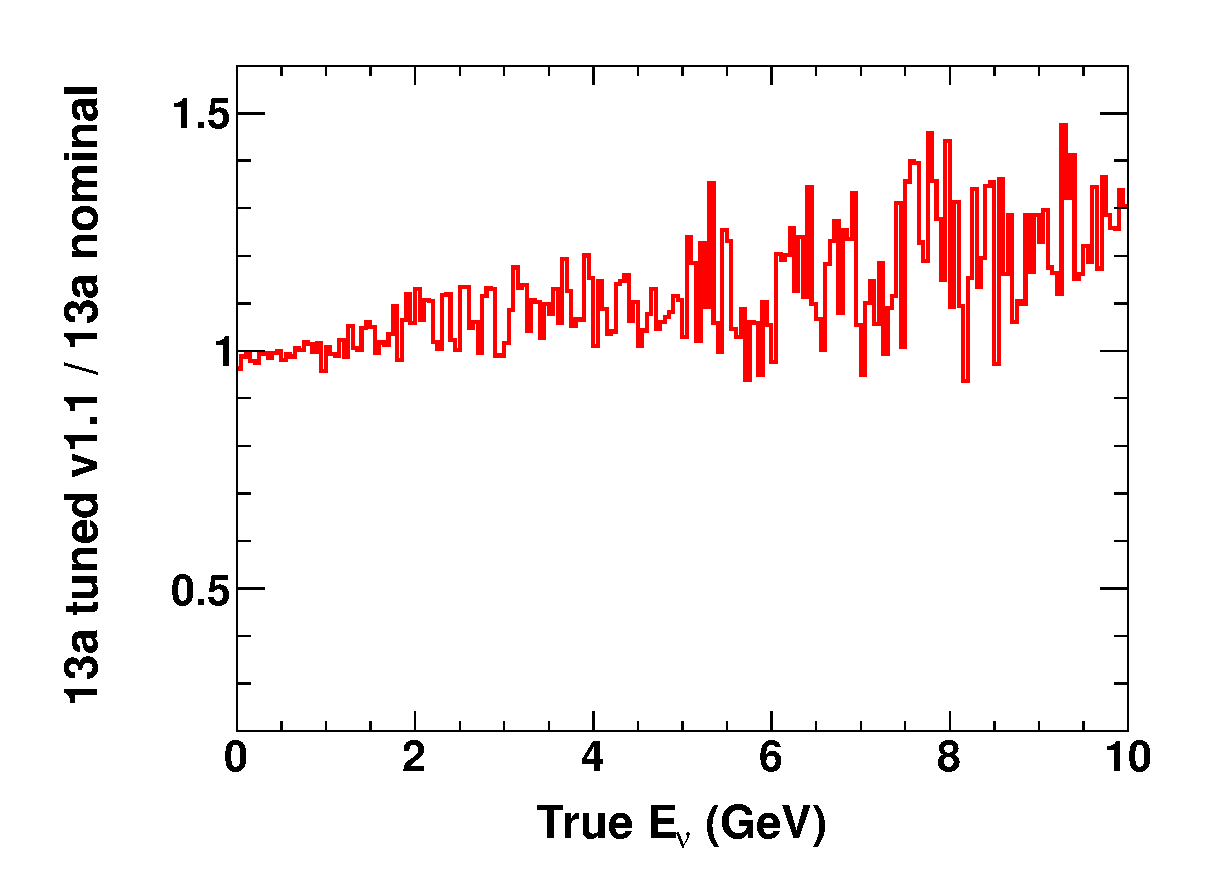
\includegraphics[width=18pc]{./images/flux/flux_ratio_13av1p1_to_13anom_numu.eps}
\caption {
  $\nu_\mu$ 13a\_v1.1 Run 5c-6e flux tuning weights applied to nominal $\nu_\mu$ and oscillated-$\nu_e$ MC templates \cite{FluxTuning13a}.}
\label{fig:na61_weights:numu}
\end{minipage}
\hspace{0.06\linewidth}
\begin{minipage}[t]{0.48\linewidth}
\center
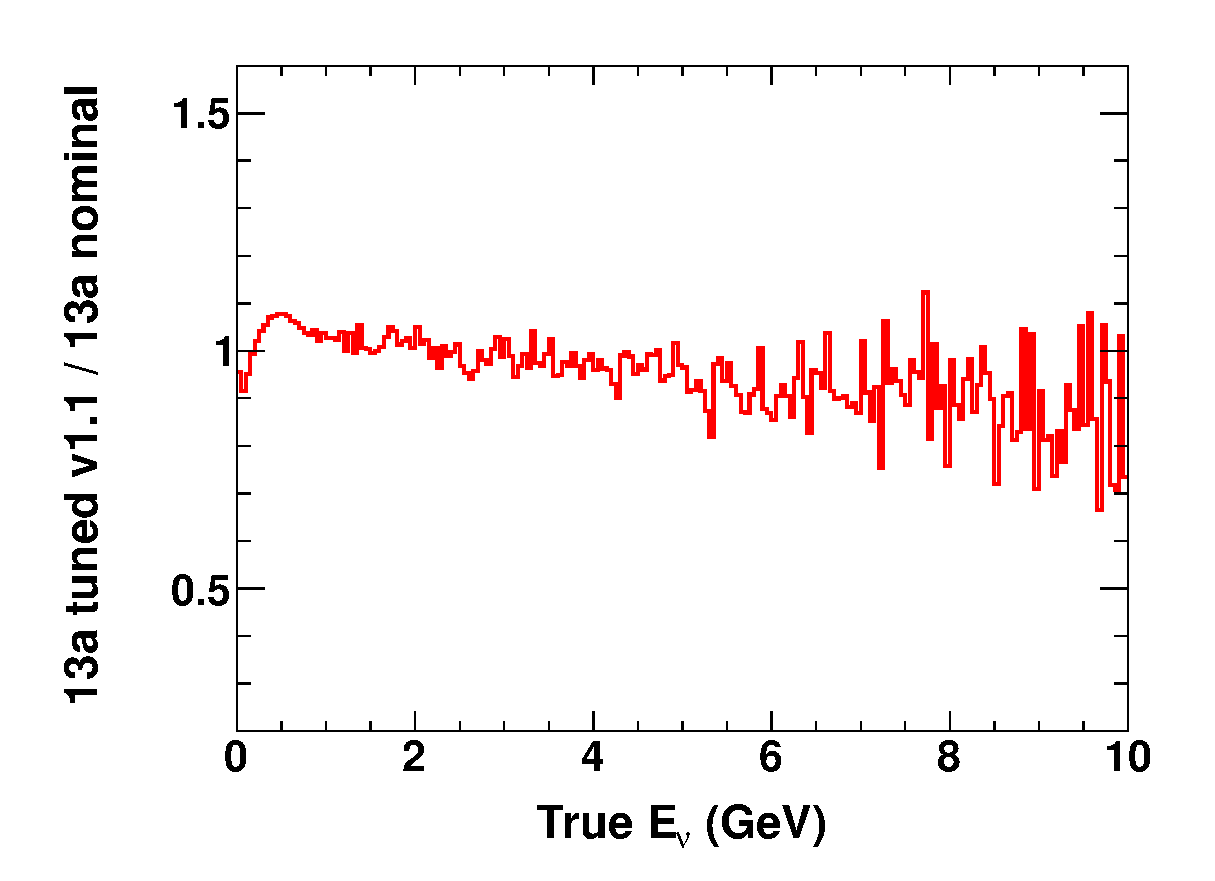
\includegraphics[width=18pc]{./images/flux/flux_ratio_13av1p1_to_13anom_numubar.eps}
\caption {
  $\bar{\nu}_\mu$ 13a\_v1.1 Run 5c-6e flux tuning weights applied to nominal $\bar{\nu}_\mu$ and oscillated-$\bar{\nu}_e$ MC templates \cite{FluxTuning13a}.}
\label{fig:na61_weights:numubar}
\end{minipage}
\vfill
\begin{minipage}[t]{0.48\linewidth}
\center
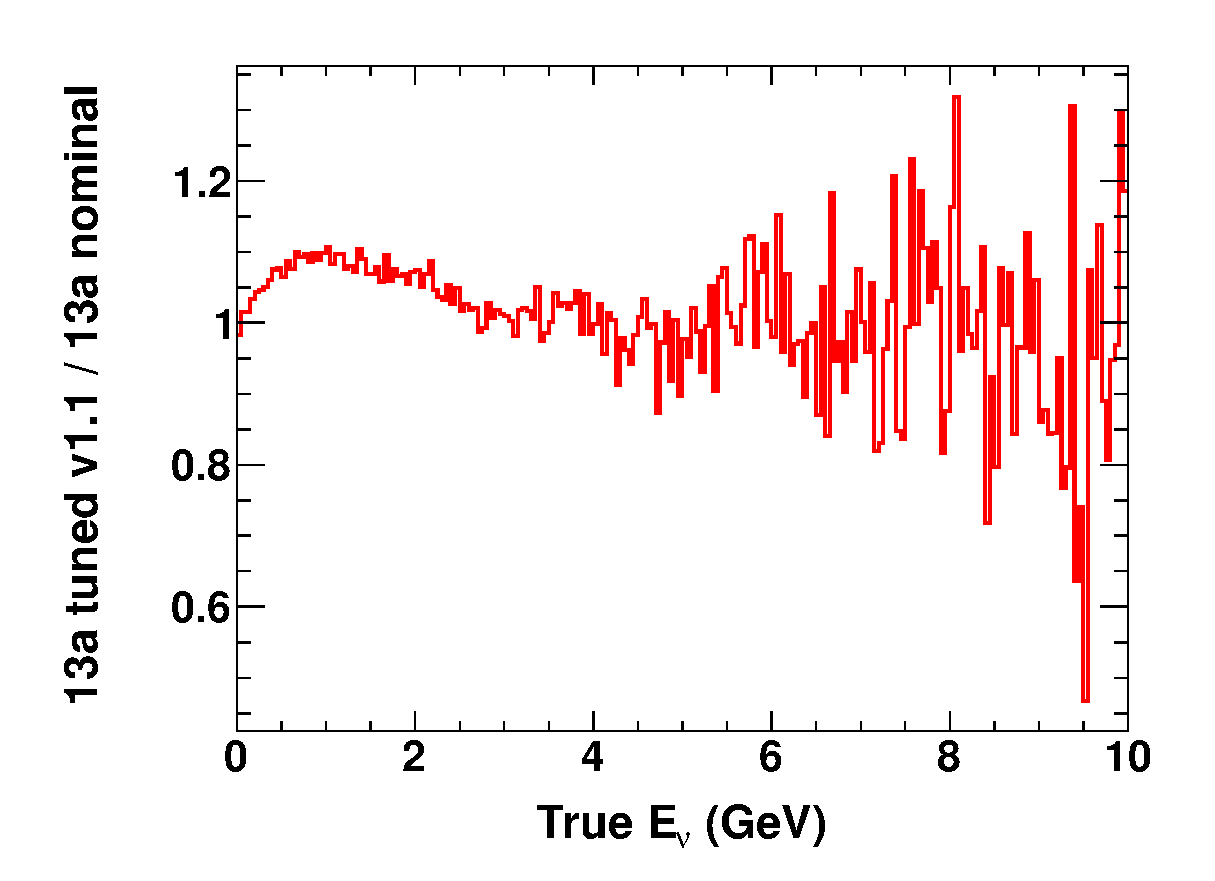
\includegraphics[width=18pc]{./images/flux/flux_ratio_13av1p1_to_13anom_nue.eps}
\caption {
  $\nu_e$ 13a\_v1.1\ Run 5c-6e flux tuning weights applied to nominal $\nu_e$ MC templates \cite{FluxTuning13a}.}
\label{fig:na61_weights:nue}
\end{minipage}
\hspace{0.06\linewidth}
\begin{minipage}[t]{0.48\linewidth}
\center
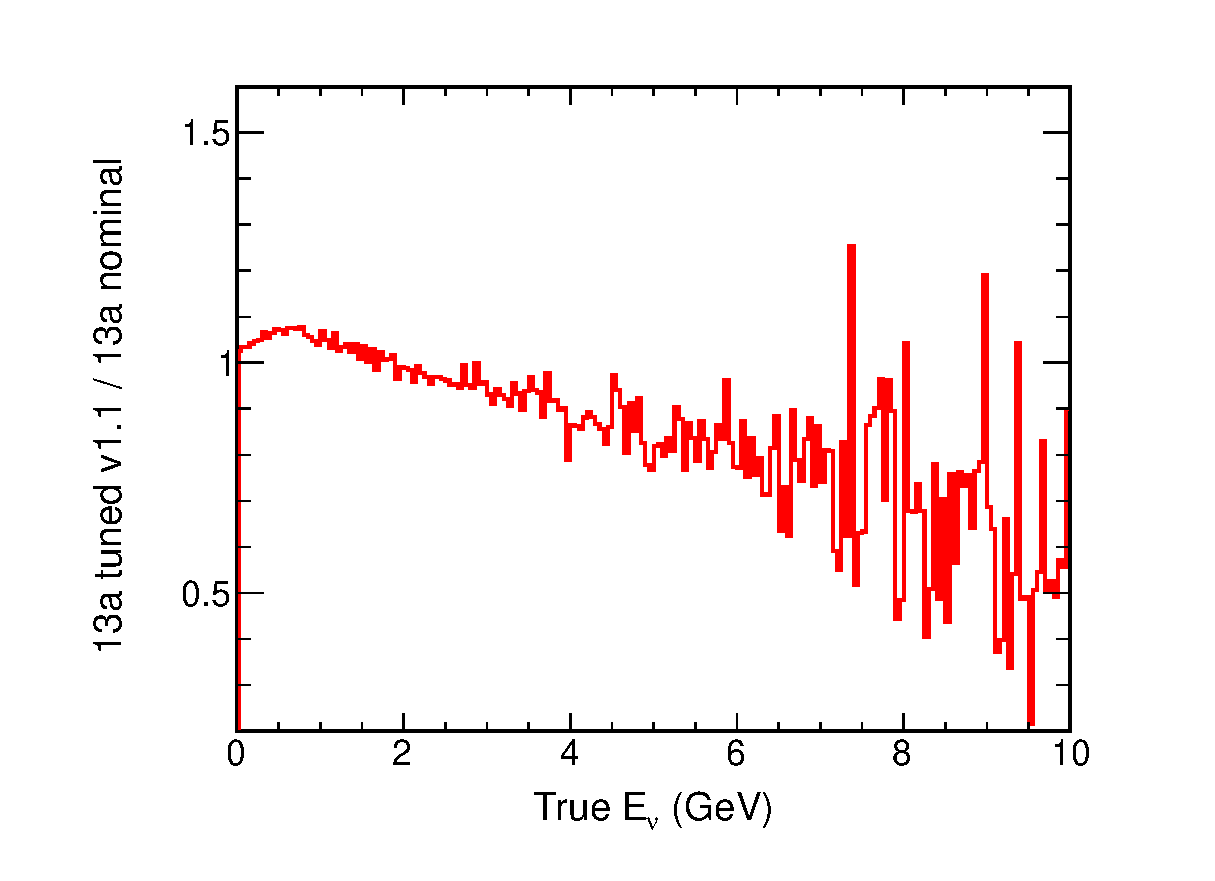
\includegraphics[width=18pc]{./images/flux/flux_ratio_13av1p1_to_13anom_nuebar.eps}
\caption {
  $\bar{\nu}_e$ 13a\_v1.1 Run 5c-6e flux tuning weights applied to nominal $\bar{\nu}_e$ MC templates \cite{FluxTuning13a}.}
\label{fig:na61_weights:nuebar}
\end{minipage}
\end{figure*}

%....................................................................................................................
%....................................................................................................................

\subsection {Applying flux and cross-section (BANFF) tuning based on ND280 data}
\label{sec:banff_weights}

The BANFF group has made a fit of the $\bar{\nu}_\mu$ and  $\nu_\mu$ CC0$\pi$-like, CC1$\pi$-like and CC other ND280 samples 
to find the best-fit values of the flux normalisation and cross-section parameters\cite{BANFF2015}. This 
analysis uses these best-fit values to reweight the NA61-tuned MC templates, and the templates obtained after this second 
reweighting will be denoted the {\em BANFF-tuned} MC templates in this document.
A list of BANFF parameters, their best-fit values and their 1$\sigma$ prefit and postfit errors is given in Tab.~\ref{tab:banff_uncertainties}.

The effects of the BANFF tune on the predicted reconstructed energy spectrum of single $\mu$-like ring events is discussed 
in Sec.~\ref{sec:nominal_and_tuned_predictions} (see Figs.~\ref{fig:1Rmu_spectrum_w_and_wo_banff_weights} and Tabs.~\ref{tab:nsk_nominal_no_osc} and~\ref{tab:nsk_nominal_osc}. 
%....................................................................................................................
%....................................................................................................................

\subsection{Applying neutrino oscillations}
\label{sec:applying_oscillations}

The MC templates are constructed from the unoscillated MC samples and must be weighted with the appropriate survival or oscillation 
probability. Oscillations are applied as a function of true energy to the
%  $\bar{\nu}_{\mu}$ CCQE,
%  $\bar{\nu}_{\mu}$ CC1$\pi$,
%  $\bar{\nu}_{\mu}$ CC coherent,
%  $\bar{\nu}_{\mu}$ CC other,
%  $\nu_{\mu}$ CCQE,
%  $\nu_{\mu}$ CC1$\pi$,
%  $\nu_{\mu}$ CC coherent,
%  $\nu_{\mu}$ CC other,
%  $\bar{\nu}_{e}$ CCQE,
%  $\bar{\nu}_{e}$ CC1$\pi$,
%  $\bar{\nu}_{e}$ CC coherent,
%  $\bar{\nu}_{e}$ CC other
%  $\nu_{e}$ CCQE,
%  $\nu_{e}$ CC1$\pi$,
%  $\nu_{e}$ CC coherent,
%  $\nu_{e}$ CC other,
%  oscillated $\bar{\nu}_{\mu} \rightarrow \bar{\nu}_{e}$ CCQE,
%  oscillated $\bar{\nu}_{\mu} \rightarrow \bar{\nu}_{e}$ CC1$\pi$,
%  oscillated $\bar{\nu}_{\mu} \rightarrow \bar{\nu}_{e}$ CC coherent,
%  oscillated $\bar{\nu}_{\mu} \rightarrow \bar{\nu}_{e}$ CC other,
%  oscillated $\nu_{\mu} \rightarrow \nu_{e}$ CCQE,
%  oscillated $\nu_{\mu} \rightarrow \nu_{e}$ CC1$\pi$,
%  oscillated $\nu_{\mu} \rightarrow \nu_{e}$ CC coherent,
%  oscillated $\nu_{\mu} \rightarrow \nu_{e}$ CC other,
%  oscillated $\nu_{e} \rightarrow \nu_{\mu}$ CCQE,
%  oscillated $\nu_{e} \rightarrow \nu_{\mu}$ CC1$\pi$,
%  oscillated $\nu_{e} \rightarrow \nu_{\mu}$ CC coherent and
%  oscillated $\nu_{e} \rightarrow \nu_{\mu}$ CC other
  MC templates for all CC interactions.

In this $\bar{\nu}_{\mu}$-disappearance analysis, two separate sets of oscillation parameters are used when calculating 
these survival or oscillation probabilities. The MC templates calculated from the $\bar{\nu}_{\mu}$ MC sample are weighted 
with P($\bar{\nu}_{\mu}\rightarrow\bar{\nu}_{\mu}$), with this survival probability being calculated using the first set of 
oscillation parameters, namely $\sin^{2}\overline{\theta}_{23}$, $\sin^{2}\overline{\theta}_{12}$, $\sin^{2}\overline{\theta}_{13}$, 
$|\overline{\Delta m}^{2}_{32}|$ (normal hierarchy) or $|\overline{\Delta m}^{2}_{31}|$ (inverted hierarchy), 
$|\overline{\Delta m}^{2}_{21}|$ and $\delta_{CP}$. The $\bar{\nu}_{e}$ templates are weighted with P($\bar{\nu}_{e}\rightarrow\bar{\nu}_{e}$), 
while the oscillated $\bar{\nu}_{\mu} \rightarrow \bar{\nu}_{e}$ templates are weighted with P($\bar{\nu}_{\mu}\rightarrow\bar{\nu}_{e}$) 
(the sample was generated assuming 100\% of $\bar{\nu}_{\mu}$ transform to $\bar{\nu}_{e}$). Again these survival and oscillation probabilities 
are calculated using the first set of oscillation parameters. 

The $\nu_{\mu}$ templates are weighted with P($\nu_{\mu}\rightarrow\nu_{\mu}$), and this survival probability is calculated using the 
second set of oscillation parameters, which are $\sin^{2}\theta_{23}$, $\sin^{2}\theta_{12}$,
$\sin^{2}\theta_{13}$, $|\Delta m^{2}_{32}|$ (normal hierarchy) or $|\Delta m^{2}_{31}|$ (inverted hierarchy),
$|\Delta m^{2}_{21}|$ and $\delta_{CP}$. The $\nu_{e}$ templates are weighted with P($\nu_{e}\rightarrow\nu_{e}$) and the 
oscillated $\nu_{\mu} \rightarrow \nu_{e}$ templates with P($\nu_{\mu}\rightarrow\nu_{e}$), with these survival and oscillation 
probabilities being calculated using the second set of oscillation parameters.

All these survival and oscillation probabilities are computed in a 3-flavour framework including matter effects in constant-density matter
(assuming an Earth crust density of 2.6 g/cm$^{3}$).
Custom oscillation probability calculation code was developed within the {\em VALOR} analysis framework.
Details and estimates of the numerical accuracy of this code were first presented in \cite{OurRun12DisappAnalysis3Flavour},
and is also shown in Appendix A of \cite{OurRun123DisappAnalysis3Flavour}.
Comparisons between the {\em VALOR} oscillation probability calculation code and Prob3++ \cite{Prob3}, 
which is typically used by the alternative T2K oscillation analyses, are shown in Appendix B of \cite{OurRun123DisappAnalysis3Flavour}.

In the standard 3-flavour oscillation framework,
oscillations of $\nu_{e}$ and $\nu_{\mu}$ can yield $\nu_{\tau}$, while
oscillations of $\bar{\nu}_{e}$ and $\bar{\nu}_{\mu}$ can yield $\bar{\nu}_{\tau}$.
In this analysis, we neglect contributions from $\nu_{\tau}$-CC and $\bar{\nu}_{\tau}$-CC as their
energy threshold is around 3.5 GeV and their effect is negligible\footnote{
A back-of-the-envelope calculation can be found in the replies to
comments and revision history document of
\cite{OurRun123DisappAnalysis3Flavour} that gives $\ll 1\%$ $\nu_\tau$
contamination in the 1-ring $\mu$-like SuperK sample. A SuperK MC study is required
to determine whether the SuperK efficiency assumptions made there are valid.
  }.
Accordingly, this analysis uses no $\nu_{\tau}$-CC and $\bar{\nu}_{\tau}$-CC MC templates
(and, in fact, no $\nu_{\tau}$ and $\bar{\nu}_{\tau}$ SuperK MC samples are available).

It should be emphasised here that
the $\nu_{\mu}$ NC MC templates for a mode $m$ are proxies for the
NC MC templates for the mixture of $\nu_{e}$+$\nu_{\mu}$+$\nu_{\tau}$ resulting from
3-flavour $\nu_{\mu}$ oscillations for that mode $m$. The same applies to the $\bar{\nu}_{\mu}$, $\nu_{e}$ and $\bar{\nu}_{e}$ 
NC MC templates. These NC MC templates are unchanged under standard 3-flavour oscillations.% (see also Sec.~\ref{sec:}).

Also it should be noted that there are no explicit NC MC templates made from the oscillated $\bar{\nu}_{e}$ and $\nu_{e}$ 
samples. If they were used, the oscillated $\bar{\nu}_{e}$ (i.e.\ $\bar{\nu}_{e}$ coming from oscillations of $\bar{\nu}_{\mu}$) 
would be double counted since they are already included in the $\bar{\nu}_{\mu}$ NC MC templates. The same applies to oscillated 
$\nu_{e}$.

%....................................................................................................................
%....................................................................................................................

\subsection {Predictions of nominal and tuned-MC single $\mu$-like ring spectra}
\label{sec:nominal_and_tuned_predictions}

In this section, we present the expected numbers of events and single $\mu$-like ring reconstructed energy spectra in SuperK 
for various oscillation scenarios. We also present estimates of the effect of the NA61 and BANFF tunings and of assumptions 
made in the 3-flavour neutrino oscillation framework used in this analysis. Unless explicitly stated otherwise, the oscillation 
parameters are set to the values shown in Tab.~\ref{tab:osc_params_fixed_values_reactor} and the normal mass hierarchy is assumed.
All plots were generated for an integrated exposure of \TotalPot POT.

%~ The expected number of single $\mu$-like ring events is shown in Fig.\ {\color{red}???} as a function of the oscillation 
%~ parameters $\sin^{2}{\overline{\theta}_{23}}$ and $|\overline{\Delta m}^{2}_{32}|$. The expected number of events ranges from 
%~ a minimum of $\sim${\color{red}??} to more than $\sim${\color{red}??}. This illustrates the great sensitivity of the T2K 
%~ $\bar{\nu}_{\mu}$-disappearance analysis in measuring $\sin^{2}{\overline{\theta}_{23}}$ with the Run 5+6 data.

Predicted single $\mu$-like ring SuperK reconstructed energy spectra are shown in Fig.~\ref{fig:1Rmu_spectrum_and_components_no_osc} for no oscillations, 
and in Fig.~\ref{fig:1Rmu_spectrum_and_components_default_osc} for oscillations assuming the normal hierarchy, and the oscillation parameters shown in table~\ref{tab:osc_params_fixed_values_reactor}.

A MC tune derived using NA61 data is applied to the nominal MC templates, and another tune derived using the ND280 data is 
applied to the NA61-tuned templates as described in Secs.~\ref{sec:na61_weights} and~\ref{sec:banff_weights}.
The fractional difference in the expected number of single $\mu$-like ring events when switching from the nominal MC to the
NA61-tuned MC templates is shown in Fig.~\ref{fig:1Rmu_spectrum_w_and_wo_na61_weights} as a function of
the reconstructed energy.
In Fig.~\ref{fig:1Rmu_spectrum_w_and_wo_banff_weights} is shown the fractional difference in the expected number of
single-ring $\mu$-like events when switching from the NA61-tuned MC templates to the BANFF-tuned MC templates.
The effects of the NA61 and BANFF tunes on the total expected number of single-ring $\mu$-like events
and on the numbers in each of the \NMCTemplate{} component interaction modes are shown in
Tab.~\ref{tab:nsk_nominal_no_osc} for no oscillations, and in
Tab.~\ref{tab:nsk_nominal_osc} for oscillations assuming the normal hierarchy, and the oscillation parameters shown in table~\ref{tab:osc_params_fixed_values_reactor}.
Finally, the effects of the NA61 and BANFF tunes on the reconstructed energy spectrum of
single $\mu$-like ring events are shown in
Figs.~\ref{fig:1Rmu_spectrum_w_and_wo_banff_weights}.
In each case, spectra are shown for both no oscillations and for oscillations assuming the normal hierarchy, and the oscillation parameters shown in table~\ref{tab:osc_params_fixed_values_reactor}.



%...........
%
% spectra, various osc scenarios
%
\begin{figure*}[htb]
\begin{minipage}[t]{0.48\linewidth}
\center
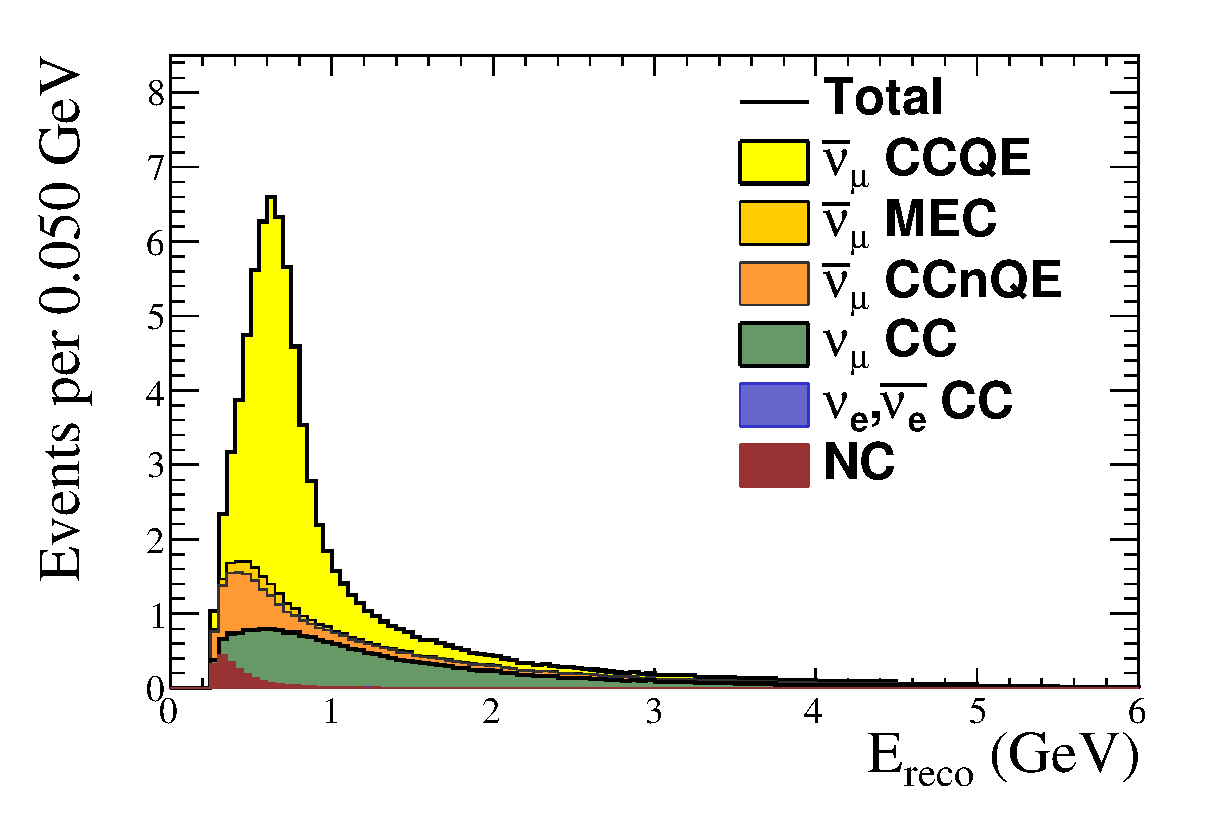
\includegraphics[width=20pc]{./images/spectrum_predictions/spectrum_unosc_grouped_prefit.eps}
\caption {
Predicted reconstructed-energy spectrum of 1 $\mu$-like ring events,
and contributions from various true neutrino reaction modes,
for no oscillations and
for an exposure of \TotalPot POT in antineutrino beam mode.
The 32 components of the spectrum are calculated separately in the actual analysis,
but, for this plot, are grouped into just 5 categories:
$\nu_{\mu}$ CCQE, $\nu_{\mu}$ CCnonQE, $\bar{\nu}_{\mu}$ CC, $\nu_{e}$/$\bar{\nu}_{e}$ CC and NC.
The spectrum was generated using the BANFF prefit MC templates.
}
\label{fig:1Rmu_spectrum_and_components_no_osc_prefit}
\end{minipage}
\hspace{0.06\linewidth}
\begin{minipage}[t]{0.48\linewidth}
\center
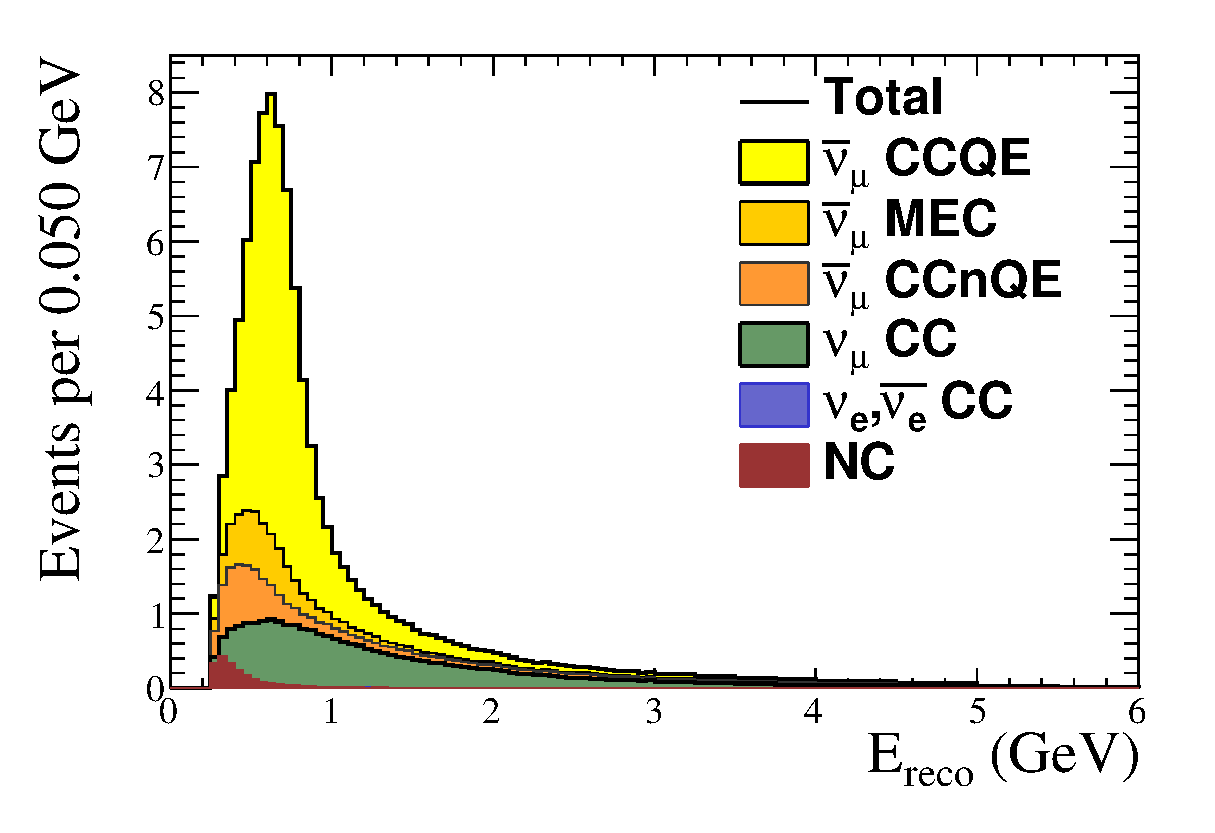
\includegraphics[width=20pc]{./images/spectrum_predictions/spectrum_unosc_grouped_postfit.eps}
\caption {
Predicted reconstructed-energy spectrum of 1 $\mu$-like ring events,
and contributions from various true neutrino reaction modes,
for no oscillations and
for an exposure of \TotalPot POT in antineutrino beam mode.
The 32 components of the spectrum are calculated separately in the actual analysis,
but, for this plot, are grouped into just 5 categories:
$\nu_{\mu}$ CCQE, $\nu_{\mu}$ CCnonQE, $\bar{\nu}_{\mu}$ CC, $\nu_{e}$/$\bar{\nu}_{e}$ CC and NC.
The spectrum was generated using the BANFF postfit-tuned MC templates.
}
\label{fig:1Rmu_spectrum_and_components_no_osc}
\end{minipage}


\end{figure*}
\begin{figure*}[htb]
\begin{minipage}[t]{0.48\linewidth}
\center
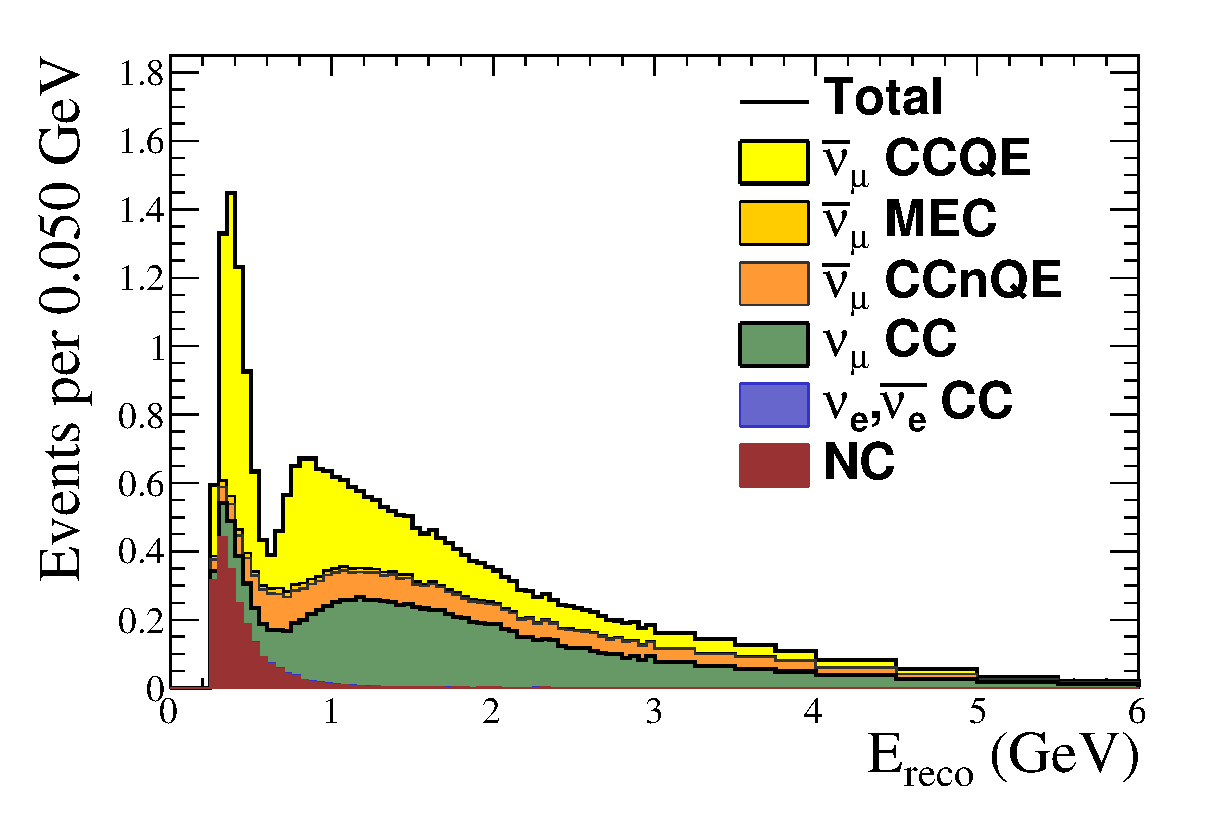
\includegraphics[width=20pc]{./images/spectrum_predictions/spectrum_osc_grouped_prefit.eps}
\caption {
Predicted reconstructed-energy spectrum of 1 $\mu$-like ring events,
and contributions from various true neutrino reaction modes,
with oscillations
for an exposure of \TotalPot POT in antineutrino beam mode.
The spectrum was generated using the BANFF prefit MC templates.
The spectrum shown was generated assuming the normal hierarchy, and the oscillation parameters shown in table~\ref{tab:osc_params_fixed_values_reactor}.
Note that the vertical axis is zoomed in by a factor of 4 compared with Fig.~\ref{fig:1Rmu_spectrum_and_components_no_osc_prefit}.
}
\label{fig:1Rmu_spectrum_and_components_default_osc_prefit}
\end{minipage}
\hspace{0.06\linewidth}
\begin{minipage}[t]{0.48\linewidth}
\center
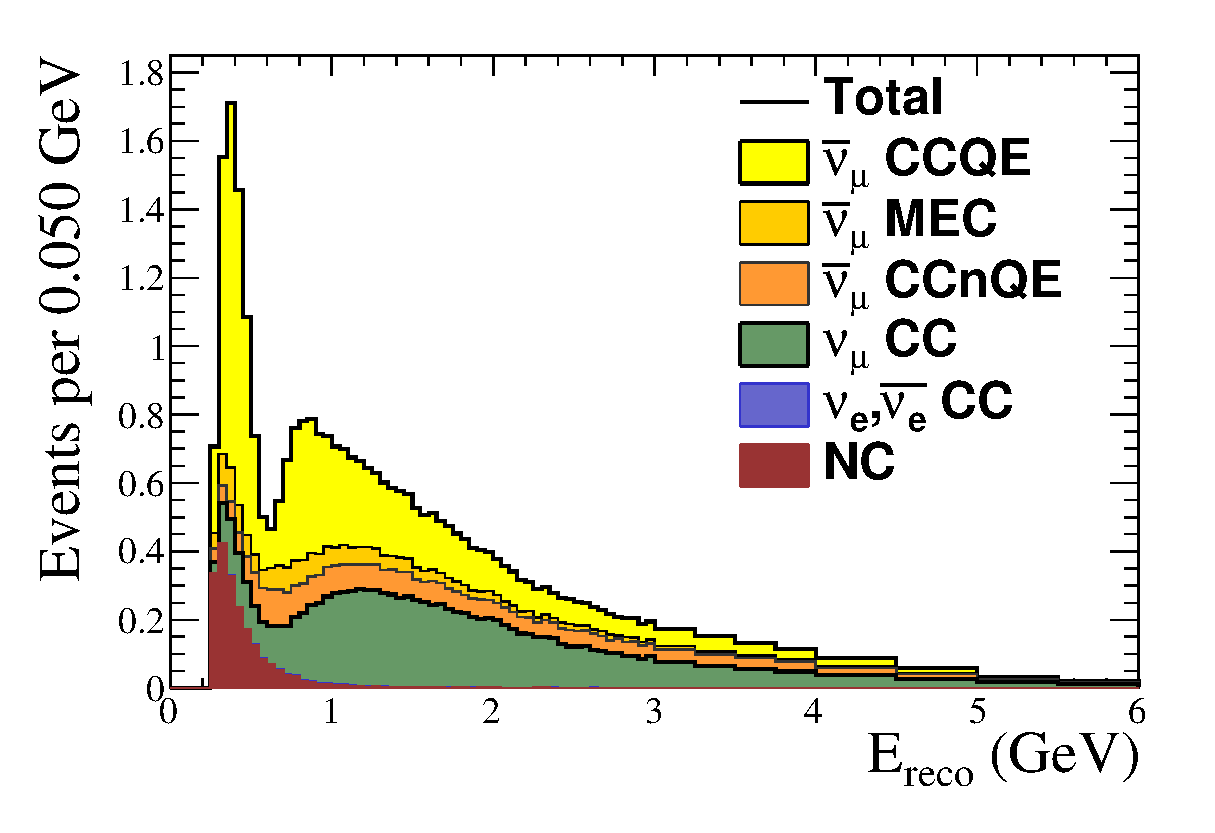
\includegraphics[width=20pc]{./images/spectrum_predictions/spectrum_osc_grouped_postfit.eps}
\caption {
Predicted reconstructed-energy spectrum of 1 $\mu$-like ring events,
and contributions from various true neutrino reaction modes,
with oscillations
for an exposure of \TotalPot POT in antineutrino beam mode.
The 32 components of the spectrum are calculated separately in the actual analysis,
but, for this plot, are grouped into just 5 categories:
$\nu_{\mu}$ CCQE, $\nu_{\mu}$ CCnonQE, $\bar{\nu}_{\mu}$ CC, $\nu_{e}$/$\bar{\nu}_{e}$ CC and NC.
The spectrum was generated using the BANFF postfit-tuned MC templates.
The spectrum shown was generated assuming the normal hierarchy, and the oscillation parameters shown in table~\ref{tab:osc_params_fixed_values_reactor}.
Note that the vertical axis is zoomed in by a factor of 4 compared with Fig.~\ref{fig:1Rmu_spectrum_and_components_no_osc}.
}
\label{fig:1Rmu_spectrum_and_components_default_osc}
\end{minipage}
\end{figure*}


%...........
%
% Plots showing the effect of tunes on Ereco spectra
%
\begin{figure*}[htb]
\center
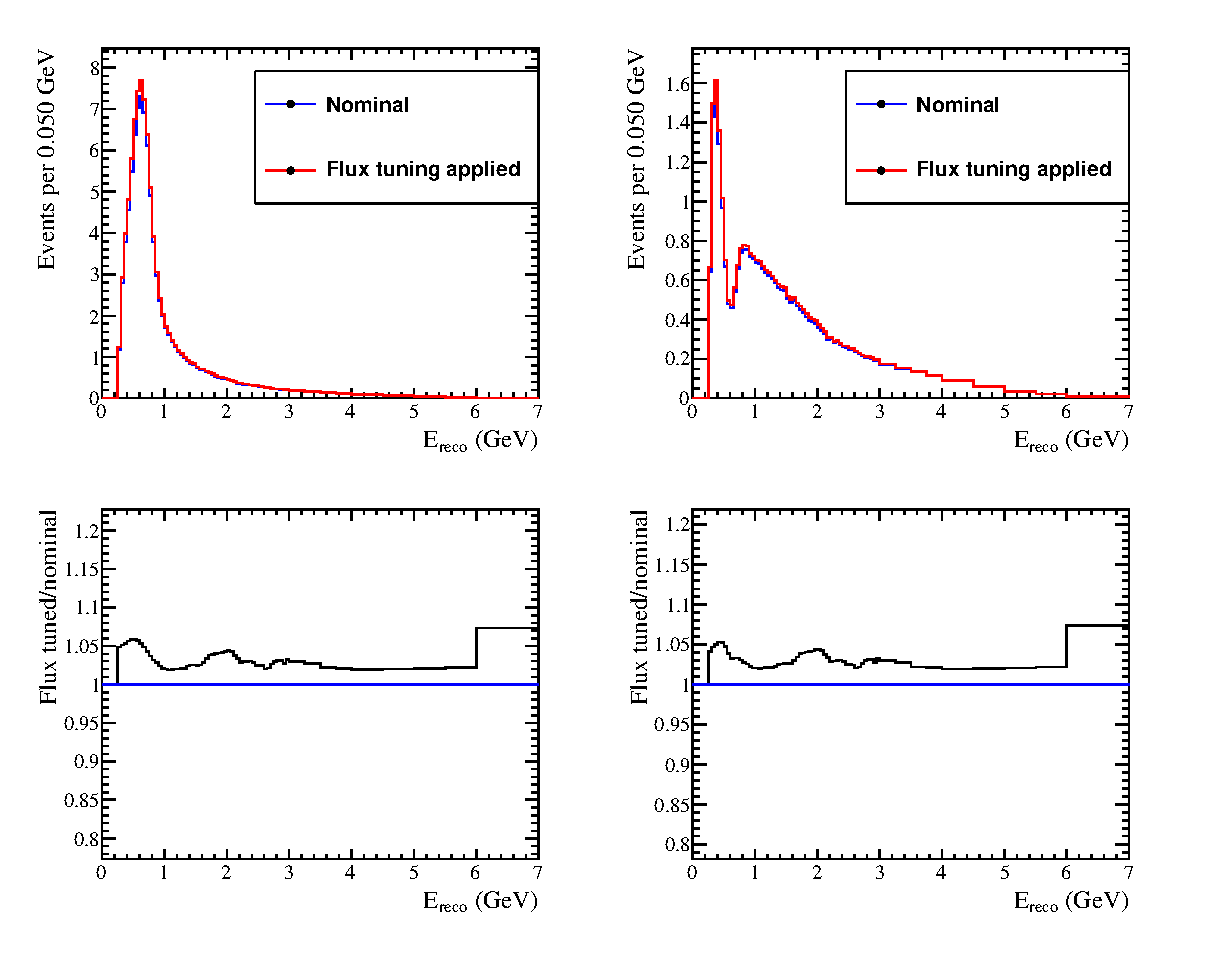
\includegraphics[width=30pc]{./images/spectrum_predictions/flux_tuning_effect.eps}
\caption {
Top: Reconstructed-energy spectrum of 1 $\mu$-like ring events,
for an exposure of \TotalPot POT in antineutrino beam mode
both with and without the effect of the NA61 flux tuning of the nominal MC templates.
The spectra are shown both for no oscillations (left)
and for oscillations assuming the normal hierarchy, and the oscillation parameters shown in table~\ref{tab:osc_params_fixed_values_reactor}.
Bottom: Ratio of flux-tuned spectrum to the nominal MC spectrum.
}
\label{fig:1Rmu_spectrum_w_and_wo_na61_weights}
\end{figure*}

\begin{figure*}[htb]
\center
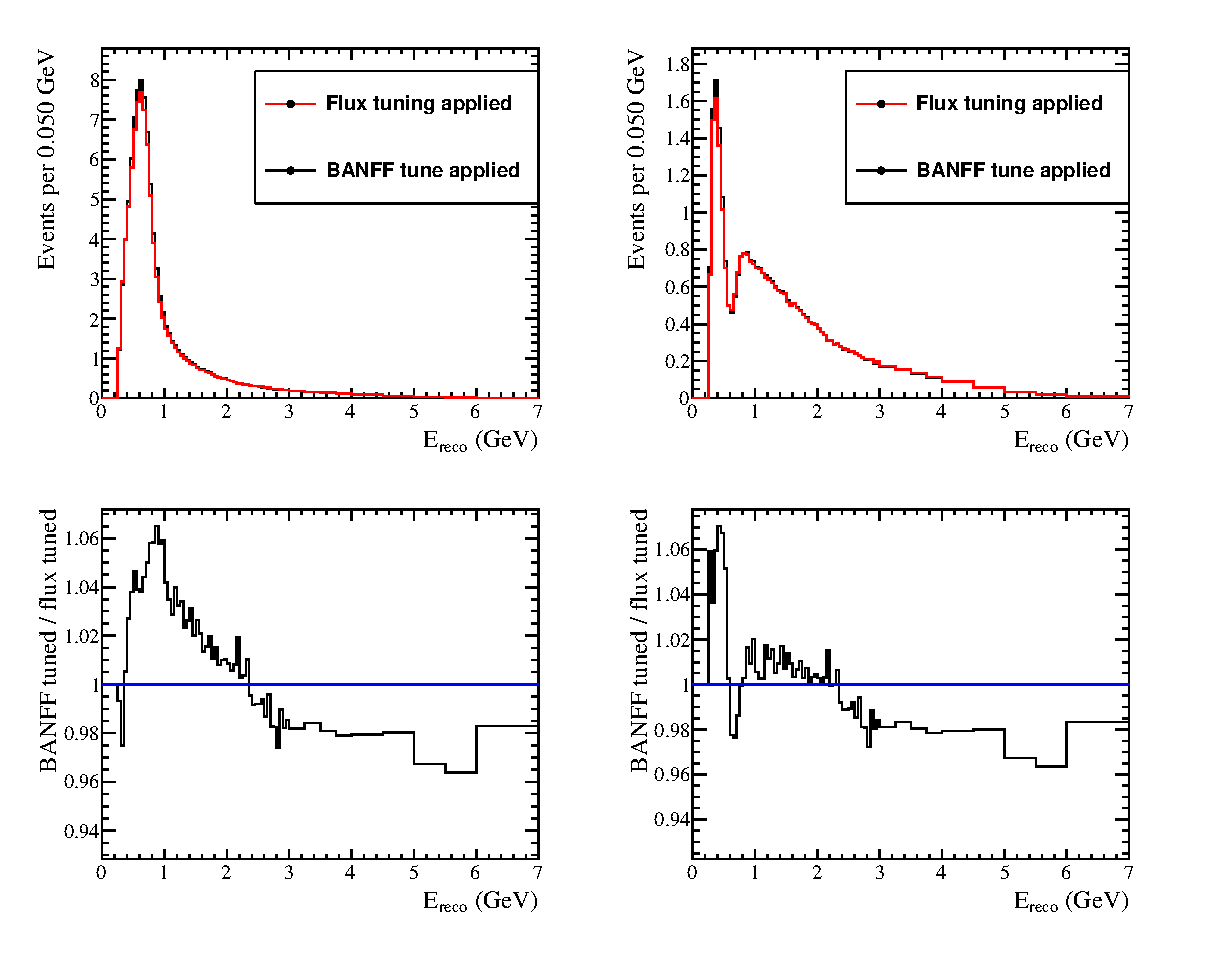
\includegraphics[width=30pc]{./images/spectrum_predictions/banff_tuning_effect.eps}
\caption {
Top: Reconstructed-energy spectrum of 1 $\mu$-like ring events,
for an exposure of \TotalPot POT in antineutrino beam mode
both with and without the effect of postfit BANFF flux and cross-section tuning on the NA61-tuned flux MC templates.
The spectra are shown both for no oscillations (left)
and for oscillations assuming the normal hierarchy, and the oscillation parameters shown in table~\ref{tab:osc_params_fixed_values_reactor}.
Bottom: Ratio of BANFF-tuned spectrum to the flux-tuned spectrum.
}
\label{fig:1Rmu_spectrum_w_and_wo_banff_weights}
\end{figure*}
